%\documentclass[handout]{beamer}
\documentclass{beamer}

\usepackage{bsymb}
\usepackage{b}
\usepackage{xcolor}

% Purpose of modelling?

% difference between axioms and invariants?
% can macine have axioms and vice versa

% why state invariants explicitly
% explain keywords

% ctr := ctr-1  versus  ctr=ctr-1

% explain skip

\mode<presentation>
{
    	%\usetheme{Warsaw}
	\setbeamertemplate{footline}
	{\centerline{\insertframenumber/\inserttotalframenumber}}
} 


\title{Event-B Example}

\author{Michael Butler, from an example by Mike Poppleton}

\institute{ University of Southampton }



\begin{document}



\begin{frame}

\titlepage

\end{frame}






\begin{frame}

\frametitle{Port Management System}

\begin{enumerate}

\item A shipping port provides a limited number of \alert{quays} at which \alert{ships} may \alert{dock}.  A quay can hold one ship \\[2ex]

\item Each ship belongs to a \alert{class} (denoting its physical berthing requirements, eg length, draught) \\[2ex]

\item A ship can only dock at a quay supporting that class 



\end{enumerate}



\end{frame}











\begin{frame} \frametitle{Class diagram for the port management  system}

  \begin{center}
    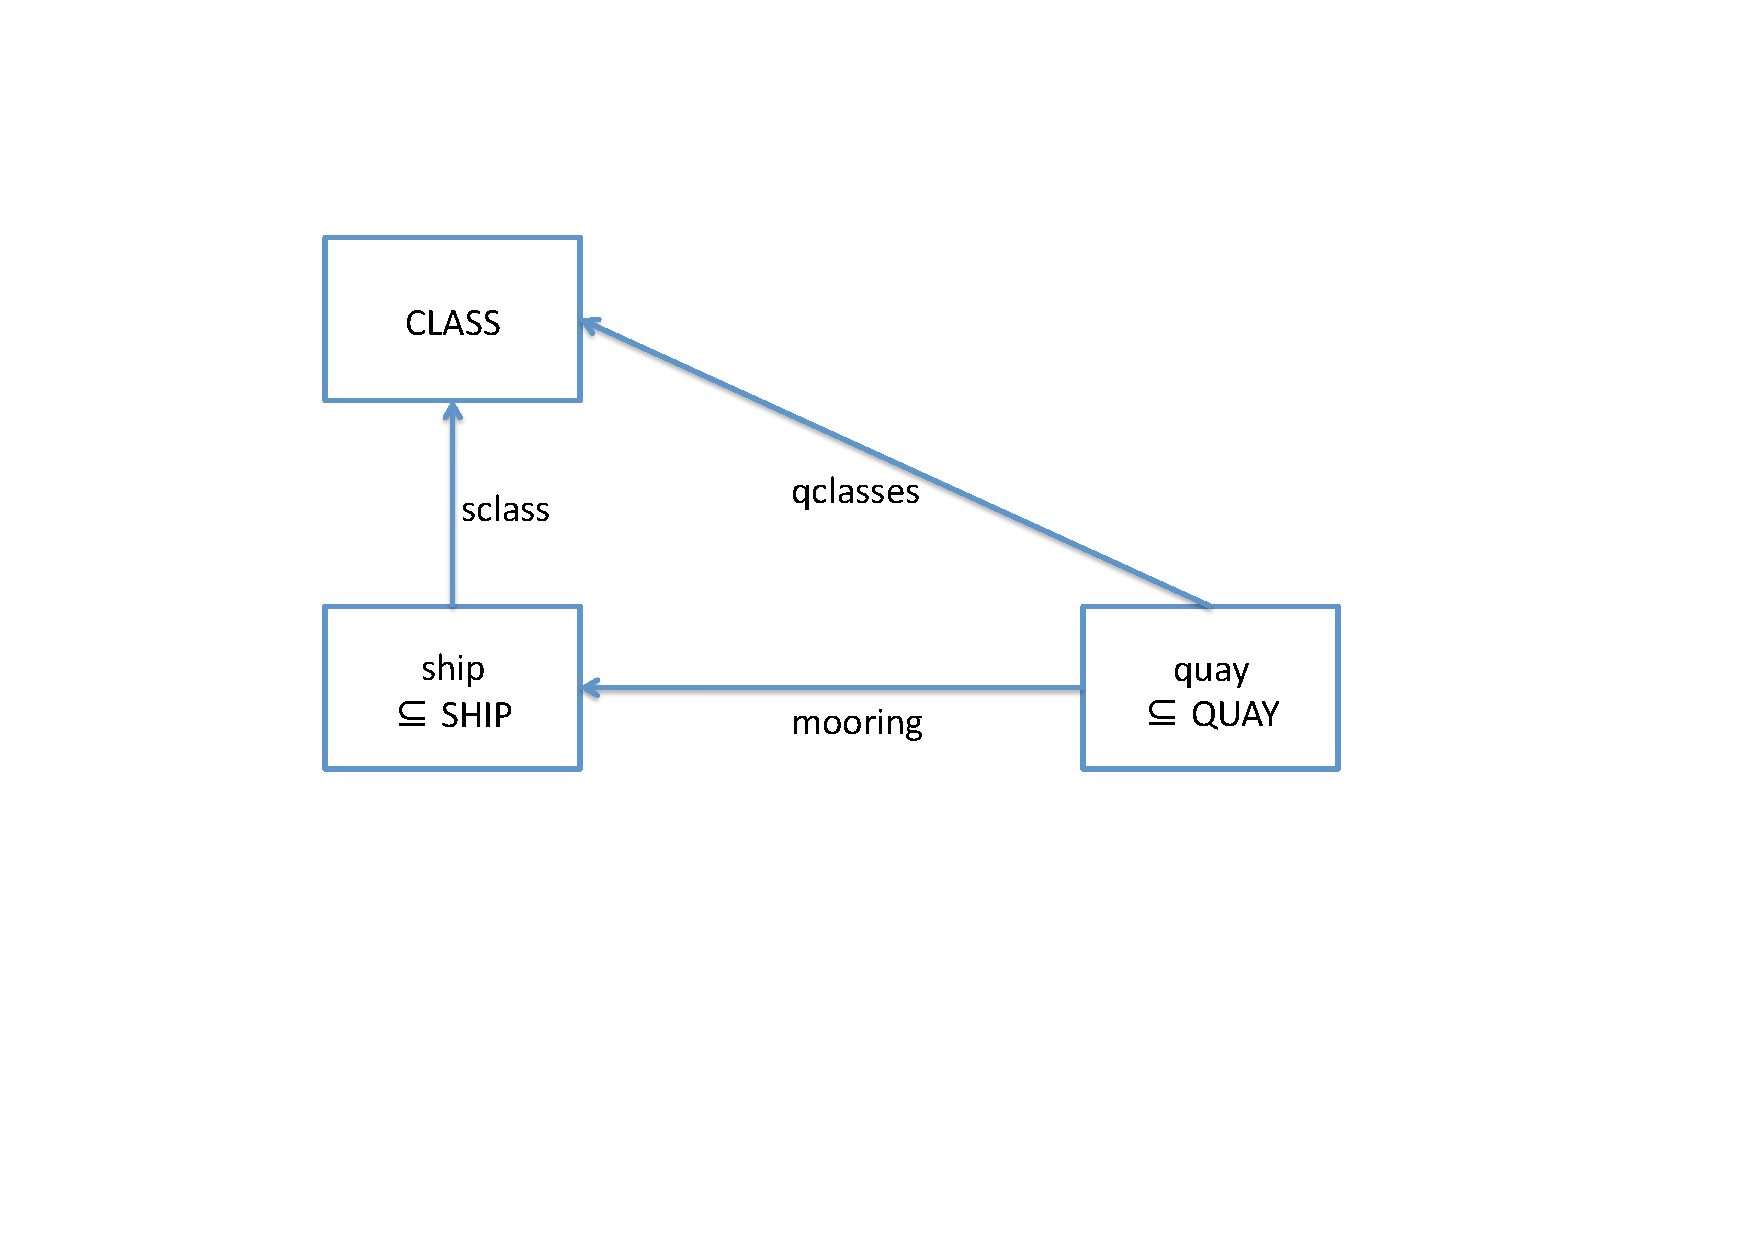
\includegraphics[scale=.5]{ship1.pdf}
  \end{center}

\end{frame}







\begin{frame}

\frametitle{Injective Functions}

\alert{One-to-one} function:
different domain elements are mapped to different range elements. 

In other words, in \alert{inverse is also a function}.

~

To declare $f$ as an injective function:
\[
     \mbox{\fbox{$~f ~\in~ X\pinj Y~$}}
\]

This is defined in terms of the inverse of $f$ as follows:

\begin{center}
\begin{tabular}{|c|c|}
\hline
Predicate & Definition \\[2pt] \hline
~&\\
$~~f ~\in~ X\pinj Y~~$ &  $~f ~\in~ X\pfun Y ~~\land~~f^{-1} \in Y\pfun X~$  \\
~&\\ \hline\end{tabular}
\end{center}


\end{frame}




\begin{frame} \frametitle{Class diagram with subsetting (inheritance)}

  \begin{center}
    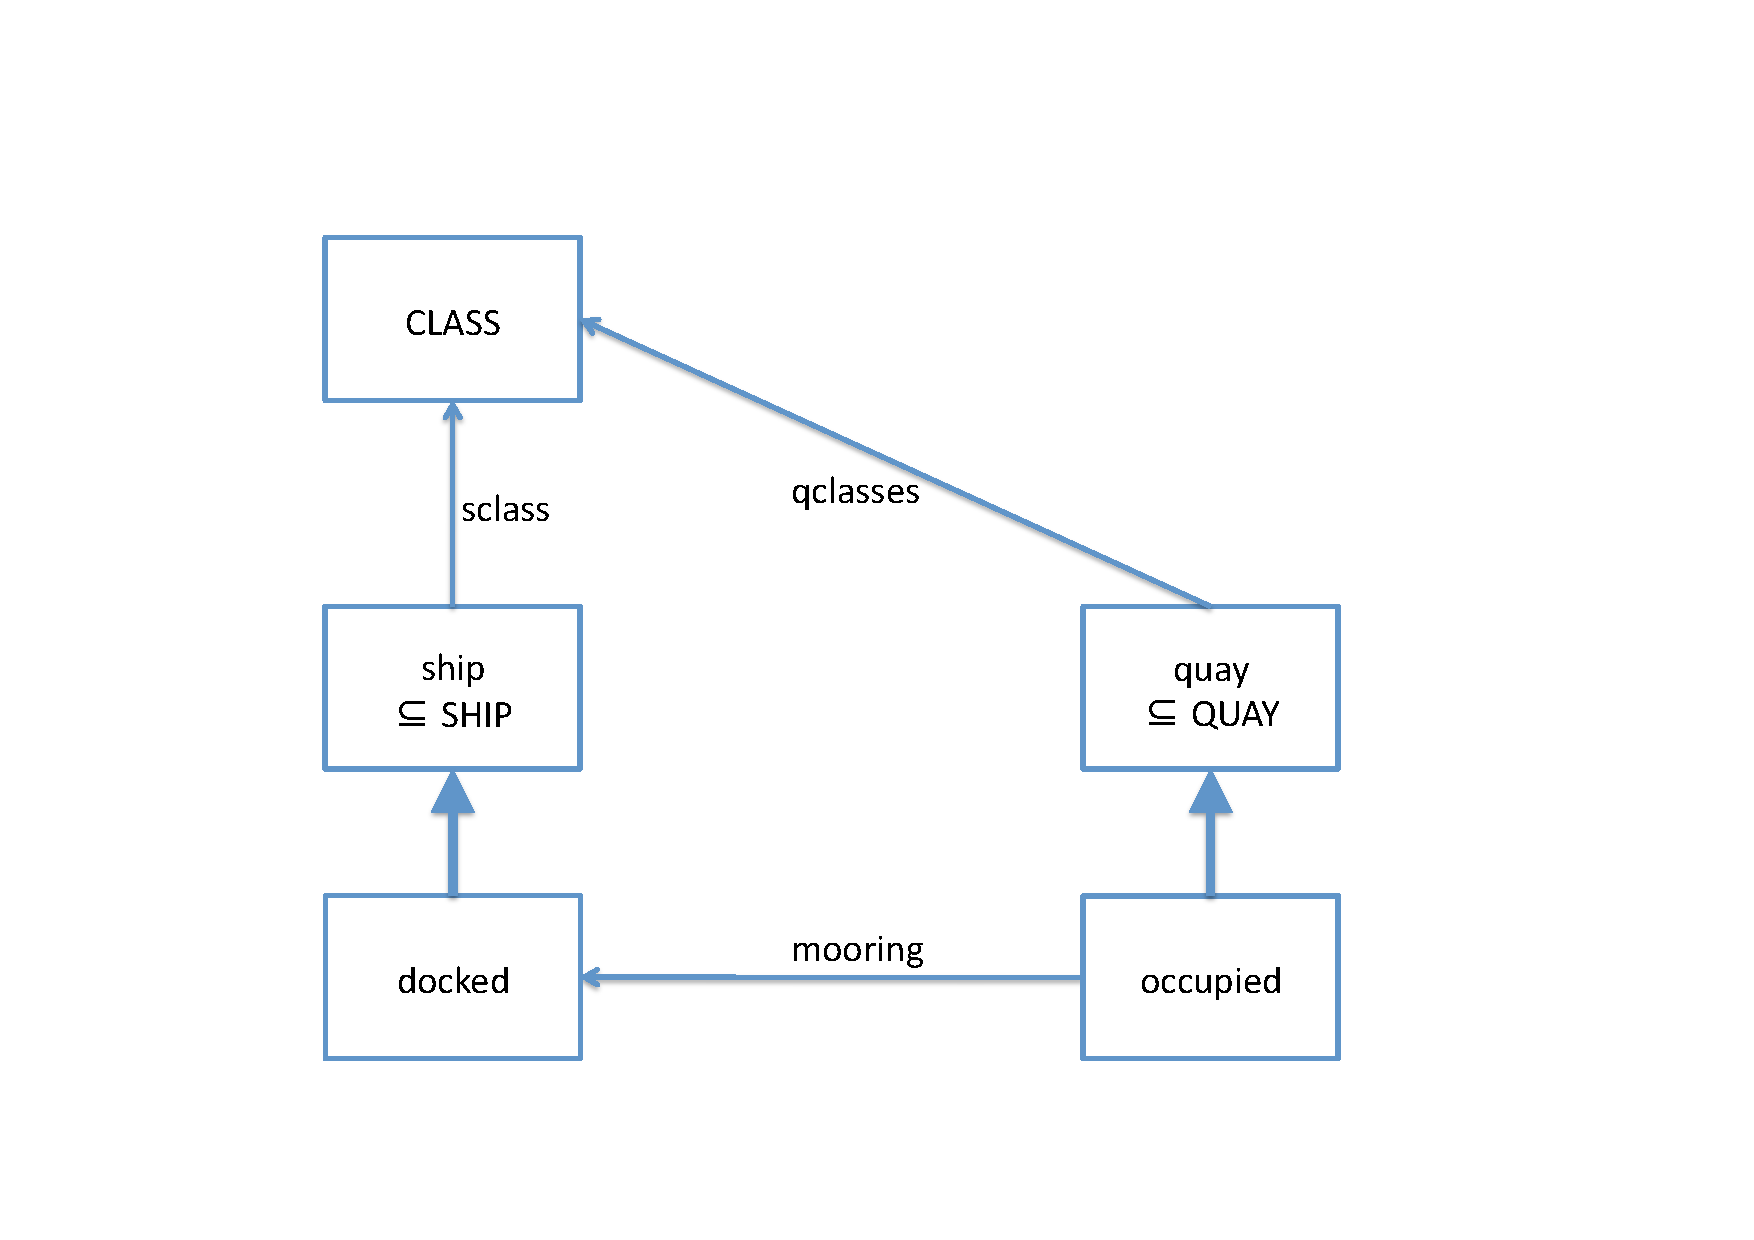
\includegraphics[scale=.5]{ship2.pdf}
  \end{center}

\end{frame}









\begin{frame}

\frametitle{Total Injective Functions}

Just as for standard total functions, we can declare an injective funciton to be
 \alert{total on some set}.



~

To declare $f$ as a total injective function:
\[
     \mbox{\fbox{$~f ~\in~ S \tinj Y~$}}
\]

This is defined i as follows:

\begin{center}
\begin{tabular}{|c|c|}
\hline
Predicate & Definition \\[2pt] \hline
~&\\
$~~f ~\in~ S \tinj Y~~$ &  $~f ~\in~ S \pinj Y ~~\land~~dom(f) =S ~$  \\
~&\\ \hline\end{tabular}
\end{center}


\end{frame}





\begin{frame}

\frametitle{Extending the Port Management System}

\begin{enumerate}


\item Besides a class, each ship has a number of \alert{processing requirements}\\[2ex]

\item Thus a ship can only dock at a quay supporting \alert{all} its processing requirements\\[2ex]


\item  An arriving ship will either
\begin{itemize}
\item dock immediately, if a suitable quay is available, or
\item join a queue of ships waiting to berth, subject to a defined queue capacity for later docking
\end{itemize}


\end{enumerate}



\end{frame}






\end{document}



